\documentclass[xcolor=svgnames]{beamer}
\usetheme{Warsaw}
\usecolortheme{dolphin}
\usepackage[T1]{fontenc}
\usepackage{graphicx}
\newtheorem{thm}{Theorem}[section]
\newtheorem{claim}[thm]{Claim}
\newtheorem{conj}[thm]{Conjecture}
\newtheorem{cor}[thm]{Corollary}
\newtheorem{conclusion}{Conclusion}
\newtheorem{qu}[thm]{Question}
\newtheorem{remark}[thm]{Remark}
\newtheorem{prop}[thm]{Proposition}
\newtheorem{prob}[thm]{Problem}
\newtheorem{exam}[thm]{Example}
\newtheorem{defn}[thm]{Definition}
\renewcommand{\emph}[1]{\textcolor{SeaGreen}{\textbf{#1}}}
\setbeamercovered{transparent}
\setbeamertemplate{navigation symbols}{} % remove navigation symbols

\usepackage{amsmath,amsxtra,amssymb,amsthm,amsfonts}
\usepackage{mathtools}
\usepackage{bm}
\usepackage{unicode-math}
\usepackage{tikz}
\setbeamertemplate{caption}[numbered]

% nice-looking footnotes in slides
\usepackage[absolute,overlay]{textpos}
\newenvironment{reference}[2]{%
  \begin{textblock*}{\textwidth}(#1,#2)
  \footnotesize\it\bgroup\color{red!50!black}}{\egroup
\end{textblock*}}

\newcommand{\bra}[1]{\langle #1 |}
\newcommand{\ket}[1]{| #1 \rangle}
\newcommand{\braket}[2]{\langle #1 | #2 \rangle}
\newcommand{\ketbra}[2]{| #1 \rangle\langle #2 |}
\newcommand{\bb}[1]{\mathbb{#1}}
\newcommand{\cl}[1]{\mathcal{#1}}
\newcommand\iprod[2]{\ensuremath{\langle#1|#2\rangle}}
\newcommand\oprod[2]{\ensuremath{|#1\rangle\langle#2|}}
\newcommand\ip[2]{\ensuremath{\langle#1 , #2\rangle}}
\newcommand\ave[1]{\ensuremath{\langle #1\rangle}}
\newcommand\Tr{\mathop{\rm Tr}\nolimits}
\newcommand\tr{\mathop{\rm tr}\nolimits}
\newcommand\supp{\mathop{\rm supp}\nolimits}
\newcommand\range{\mathop{\rm range}\nolimits}
\newcommand\argmax{\mathop{\rm argmax}\nolimits}
\newcommand\trho{\tilde{\rho}}
\newcommand\tsigma{\tilde{\sigma}}
\newcommand{\norm}[1]{\|#1\|}
%\newcommand{\norm}[1]{\left\lvert\tinyspace#1\tinyspace\right\rvert}
\newcommand{\abs}[1]{\left\lVert\tinyspace #1 \tinyspace\right\rvert}
\newcommand{\floor}[1]{\left\lfloor #1 \right\rfloor}
\newcommand{\ceil}[1]{\left\lceil #1 \right\rceil}
\newcommand{\Innerproduct}[1]{\langle{#1}\rangle}

\newcommand{\bij}{%
  \hookrightarrow\mathrel{\mspace{-15mu}}\rightarrow
}

\makeatletter
\newcommand{\xbij}[2][]{%
  \lhook\joinrel
  \ext@arrow 0359\rightarrowfill@ {#1}{#2}%
  \mathrel{\mspace{-15mu}}\rightarrow
}
\makeatother

\usepackage{algorithm,algpseudocode}
\algnewcommand\algorithmicforeach{\textbf{for each}}
\algdef{S}[FOR]{ForEach}[1]{\algorithmicforeach\ #1\ \algorithmicdo}

\algnewcommand{\algorithmicand}{\textbf{ and }}
\algnewcommand{\algorithmicor}{\textbf{ or }}
\algnewcommand{\algorithmicnot}{\textbf{ not }}
\algnewcommand{\algorithmicbreak}{\textbf{break}}
\algnewcommand{\algorithmiccontinue}{\textbf{continue}}
\algnewcommand{\AND}{\algorithmicand}
\algnewcommand{\OR}{\algorithmicor}
\algnewcommand{\NOT}{\algorithmicnot}
\algnewcommand{\BREAK}{\algorithmicbreak}
\algnewcommand{\CONTINUE}{\algorithmiccontinue}

\usepackage{xcolor,etoolbox}
\algrenewcommand\algorithmiccomment[1]{\hfill{\color{gray}\(\triangleright\)
#1}}

\makeatletter
\newcommand{\LeftComment}[1]{%
  \Statex
  {%
    \setlength\leftskip{\ALG@thistlm}%
    \noindent
    \color{gray}\(\triangleright\)\enspace#1\par%
  }%
}

\newcommand{\LeftCommentIndent}[1]{%
  \Statex
  {%
    \setlength\leftskip{\dimexpr\ALG@thistlm+\algorithmicindent}%
    \noindent
    \color{gray}\(\triangleright\)\enspace#1\par%
  }%
}
\makeatother

\def\I{\mathbb{1}}
\def\O{\mathbb{O}}
\def\C{\mathbb{C}}
\def\R{\mathbb{R}}
\def\F{\mathbb{F}}
\def\N{\mathbb{N}}
\def\Q{\mathbb{Q}}
\def\Z{\mathbb{Z}}

\def\B{\mathcal{B}}
\def\D{\mathcal{D}}
\def\Lin{\mathcal{L}}
\def\M{\mathcal{M}}
\def\S{\mathcal{S}}
\def\U{\mathcal{U}}
\def\V{\mathcal{V}}
\def\W{\mathcal{W}}
\def\X{\mathcal{X}}
\def\Y{\mathcal{Y}}

\def\a{\mathbf{a}}
\def\b{\mathbf{b}}
\def\c{\mathbf{c}}
\def\d{\mathbf{d}}
\def\e{\mathbf{e}}
\def\p{\mathbf{p}}
\def\q{\mathbf{q}}
\def\r{\mathbf{r}}
\def\u{\mathbf{u}}
\def\v{\mathbf{v}}
\def\w{\mathbf{w}}
\def\x{\mathbf{x}}
\def\y{\mathbf{y}}
\def\z{\mathbf{z}}
\def\0{\mathbf{0}}
\newcommand{\defeq}{\stackrel{\smash{\textnormal{\tiny def}}}{=}}

\newcommand{\lvnote}[1]{\textcolor{teal}{\textbf{LV:} #1}}
\newcommand{\njnote}[1]{\textcolor{teal}{\textbf{NJ:} #1}}

\title{
  Advancements in Graph Bandwidth Reduction
}
\author[\emph{L. M. B. Varona} and N. Johnston]{
  \emph{Luis M. B. Varona}\inst{1,2,3} and Nathaniel Johnston\inst{2} \\[0.25em]
  
\includegraphics[width=2.54cm]{assets/mta_logo.png} \\[-1.25em]
}
\institute[Science Atlantic MSCS 2025]{
  \inst{1}Dept. of Politics \& International Relations, MtA \\
  \inst{2}Dept. of Mathematics \& Computer Science, MtA \\
  \inst{3}Dept. of Economics, MtA \\[3em]
  Science Atlantic -- Mathematics, Statistics, \& Computer Science
  (MSCS) 2025 \\
  Cape Breton University, Sydney, NS, Canada \\[-0.5em]
}
\date{October 18, 2025}

\begin{document}

\frame{\titlepage}

%%%%%%%%%%%%%%%%%%%%%%%%%%%%%%%%%%%%%%%%
\section{Technical Background}
%%%%%%%%%%%%%%%%%%%%%%%%%%%%%%%%%%%%%%%%
%%%%%%%%%%%%%%%%%%%%%%%%%%%%%%%%%%%%%%%%
\subsection{Preliminaries and Definitions}
%%%%%%%%%%%%%%%%%%%%%%%%%%%%%%%%%%%%%%%%
\frame{
  \frametitle{Graph Bandwidth}
  \begin{defn}[Layout]
    Let $G = (V, E)$ be a graph\textsuperscript{*} with $\lvert V
    \rvert = n$. A \emph{layout} of $G$ is a bijection from $V \bij
    \{0, 1, \ldots, n - 1\}$.
  \end{defn}

  \uncover<2->{
    \begin{defn}[Graph bandwidth]
      Let $G = (V, E)$ be a graph\textsuperscript{*} with $\lvert V
      \rvert = n$. The \emph{bandwidth} $\beta(G, \pi)$ of $G$ under
      a layout $\pi$ is the maximum $k \in \{0, 1, \ldots, n - 1\}$
      such that $\lvert \pi(u) - \pi(v) \rvert \le k$ for all $\{u,
      v\} \in E$. The \emph{minimum bandwidth} $\beta(G)$ of $G$ is
      $\min \beta(G, \pi)$ taken over all layouts $\pi$.
    \end{defn}
  }

  \begin{itemize}
      \uncover<3->{
      \item Empty graphs: $\beta\left(\overline{K_n}\right) = 0$
      \item Path graphs: $\beta(P_n) = 1$
      \item Complete graphs: $\beta(K_n) = n - 1$
      }
  \end{itemize}

  \vspace*{0.5cm}
  \footnotesize{\textsuperscript{*}We use ``graph'' to refer
  specifically to a \emph{simple undirected graph}.}
}

\frame{
  \frametitle{Matrix Bandwidth}
  % Bandwidth can also be formulated as a \emph{matrix-theoretic}
  % concept (which is often more useful in numerical analysis):
  Theoreticians usually think in terms of graphs, but computational
  scientists often formulate bandwidth as a matrix-theoretic concept:
  \uncover<2->{
    \begin{defn}[Matrix bandwidth]
      Let $A$ be an $n \times n$ matrix. The \emph{bandwidth}
      $\beta(A, P)$ of $A$ under a permutation matrix $P$ is the
      maximum $k \in \{0, 1, \ldots, n - 1\}$ such that
      $\left[PAP^\mathsf{T}\right]_{i,j} \ne 0 \implies \lvert i - j
      \rvert \le k$. The \emph{minimum bandwidth} $\beta(A)$ of $A$
      is $\min \beta(A, P)$ taken over all permutation matrices $P$.
    \end{defn}
  }

  \begin{itemize}
      \uncover<3->{
      \item Often, $A$ is \emph{structurally symmetric}: $A_{i,j} = 0
        \iff A_{j,i} = 0$
      }
      \uncover<4->{
      \item If $A$ is the adjacency matrix of a graph $G$ (ignoring
        weights and diagonal entries), then $\beta(A)$ = $\beta(G)$
      }
  \end{itemize}
}

%%%%%%%%%%%%%%%%%%%%%%%%%%%%%%%%%%%%%%%%
\subsection{Examples and Applications}
%%%%%%%%%%%%%%%%%%%%%%%%%%%%%%%%%%%%%%%%
\frame{
  \frametitle{Bandwidth Reduction Example}
  \begin{figure}
    \begin{minipage}[b]{.475\textwidth}
      \vspace*{0.3cm}
      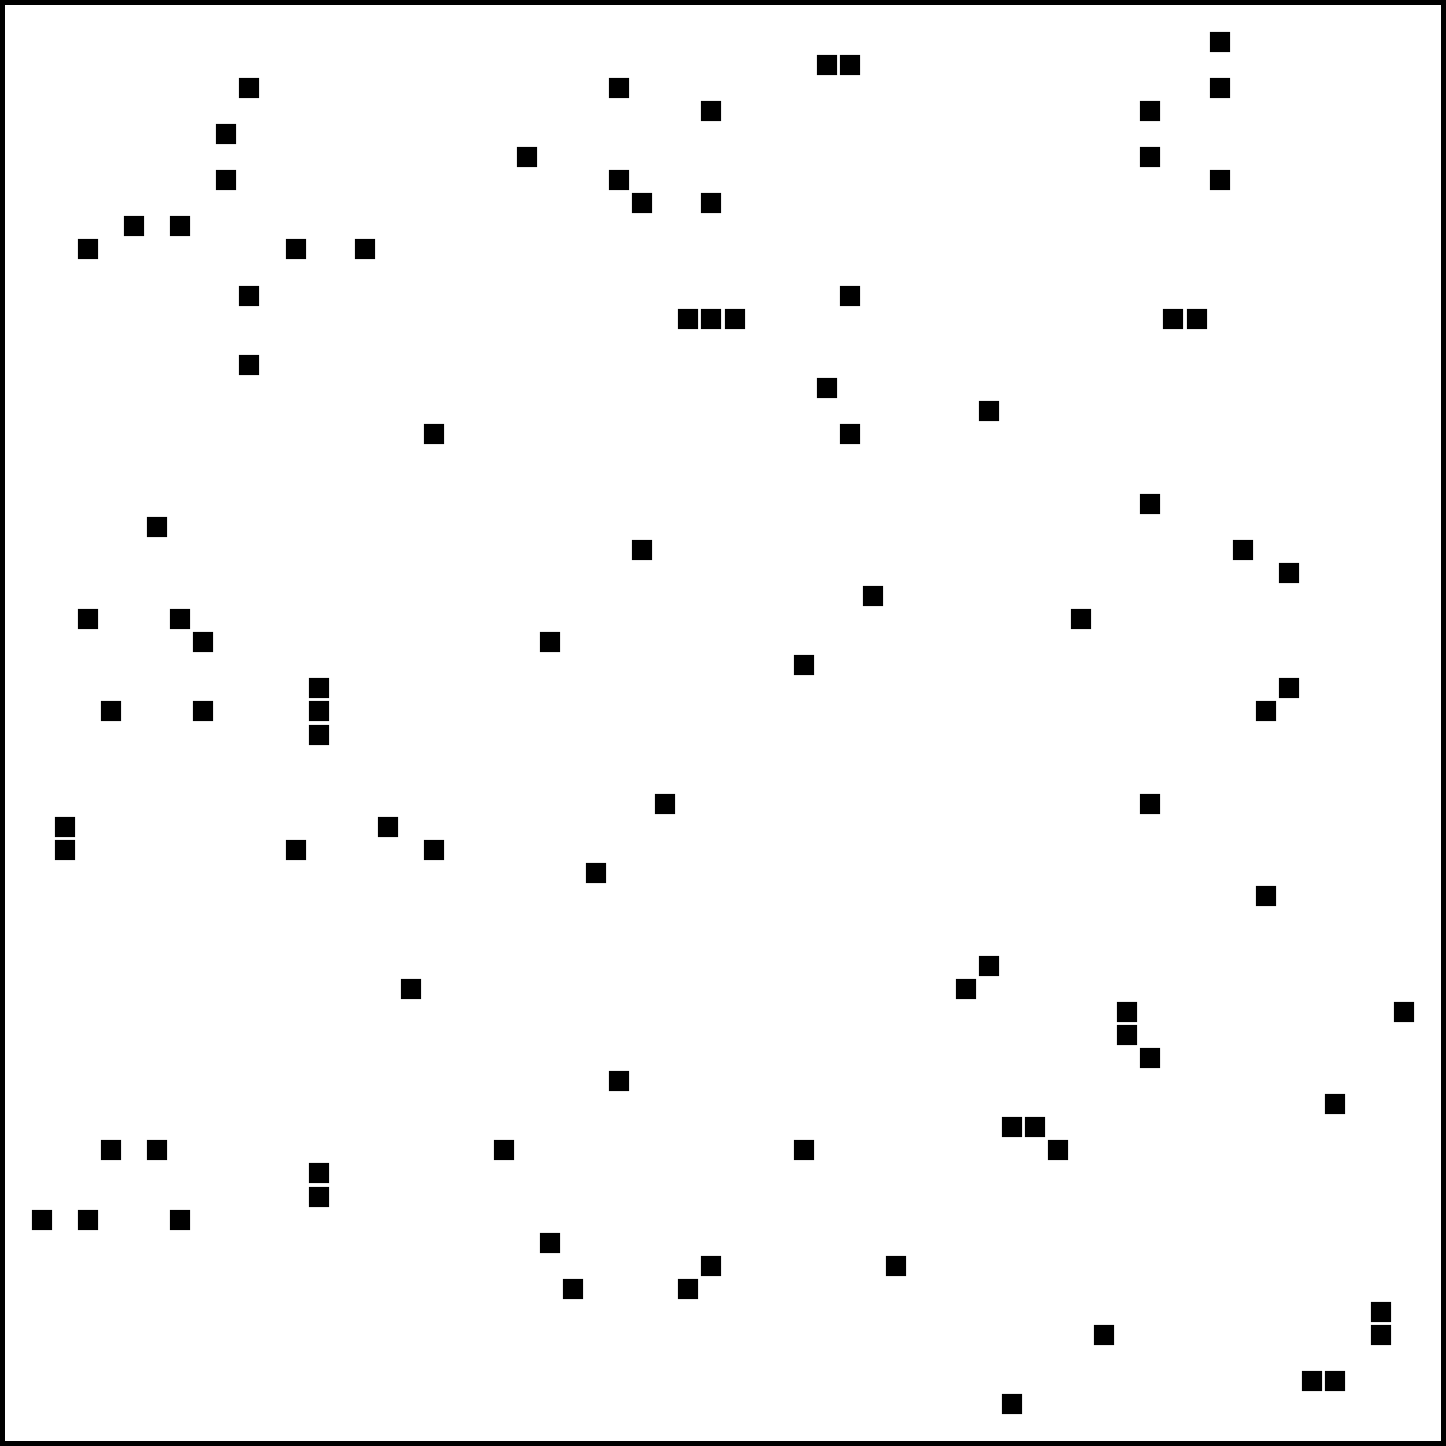
\includegraphics[height=5.2cm]{assets/highband_mat.png}
      \vspace*{-1.5em}
      \caption{A $60 \times 60$ sparse matrix with original bandwidth $51$.}
      \vspace*{1.09em}
      \label{fig:highband-mat}
    \end{minipage}\hfill
    \begin{minipage}[b]{.475\textwidth}
      \vspace*{0.5em}
      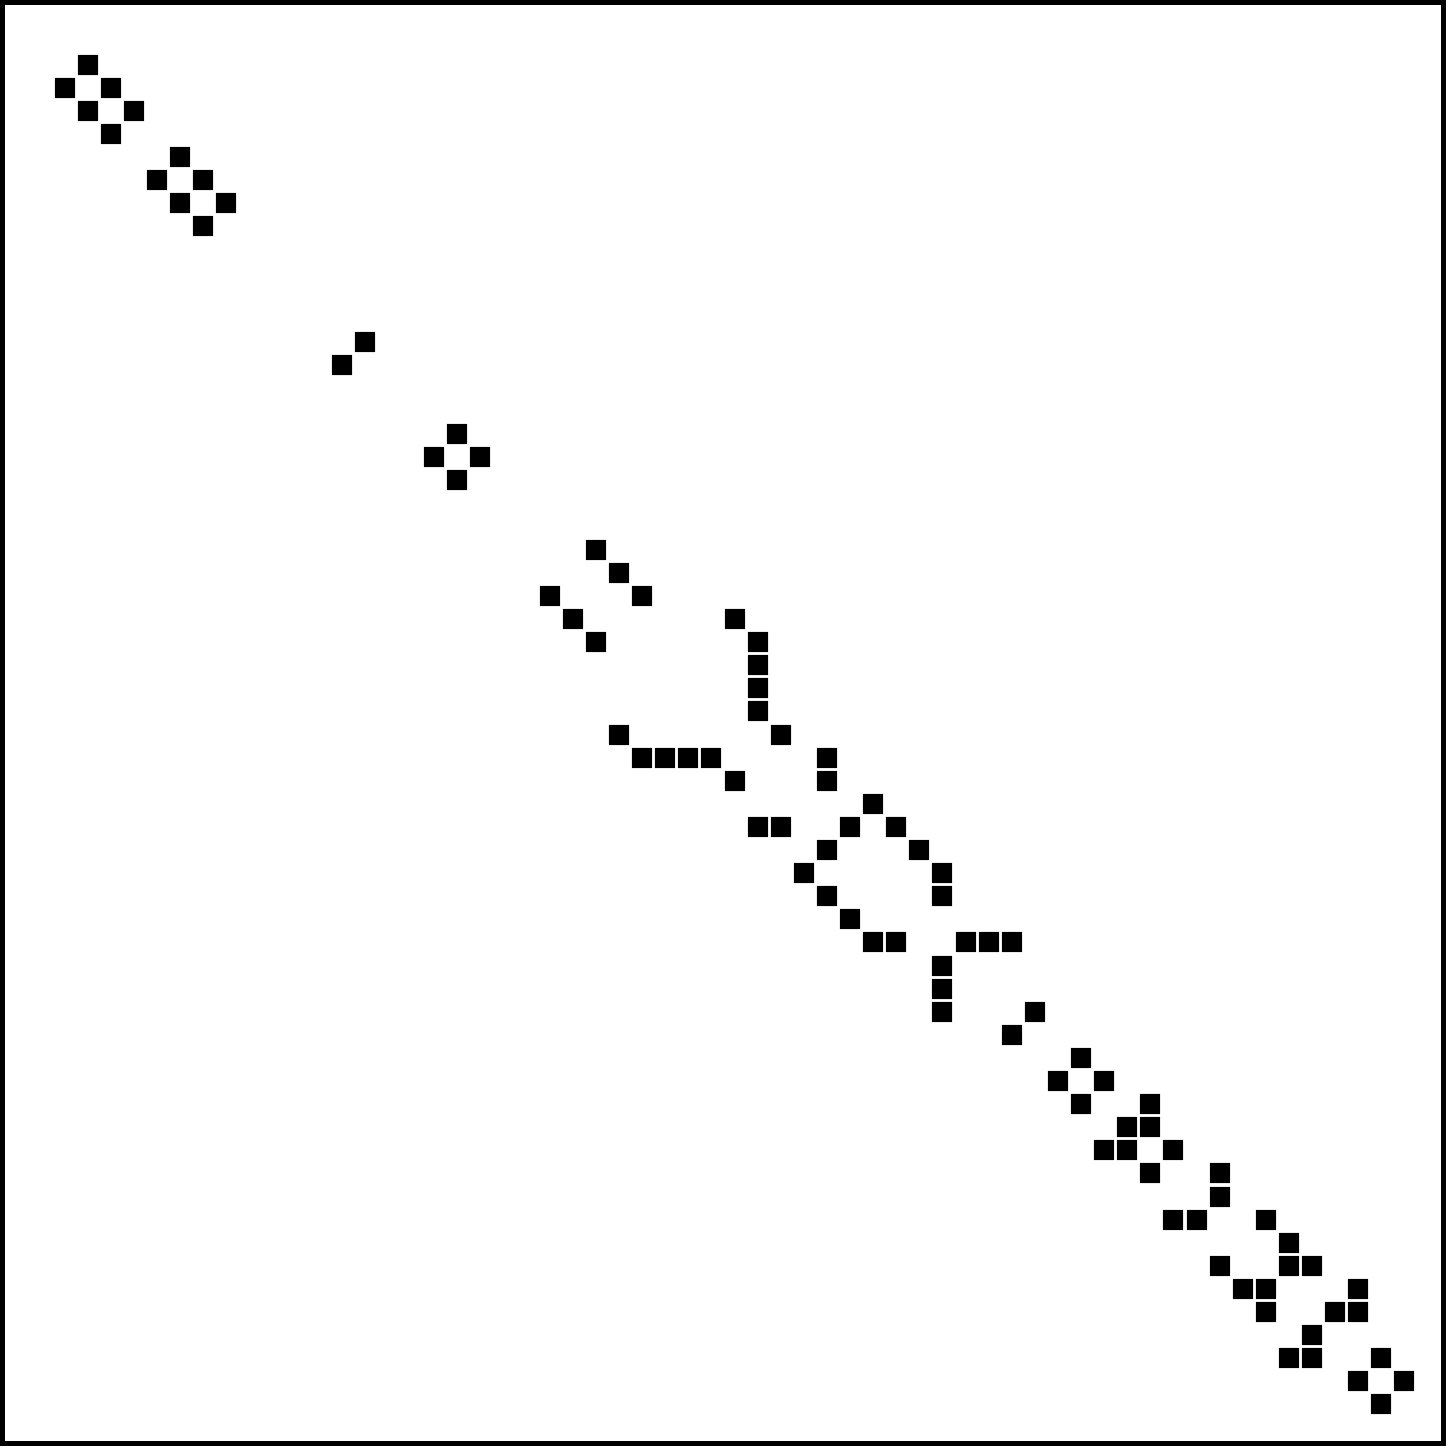
\includegraphics[height=5.2cm]{assets/lowband_mat.png}
      \vspace*{-1.5em}
      \caption{Bandwidth reduced to $5$ by the
      \emph{Gibbs--Poole--Stockmeyer} heuristic algorithm.}
      \label{fig:lowband-mat}
    \end{minipage}
  \end{figure}
}

\frame{
  \frametitle{Practical Applications}
  Applications in engineering, scientific computing, and more:
  \begin{itemize}
      \uncover<2->{
      \item approximating \emph{partial differential equations}\ldots
      }
      \uncover<3->{
      \item optimizing \emph{circuit layout}\ldots
      }
      \uncover<4->{
      \item training \emph{recurrent neural networks}\ldots
      }
      \uncover<5->{
      \item even investigating operators in \emph{quantum information theory}!
      }
  \end{itemize}

  \begin{figure}
    \centering
    \visible<3->{
      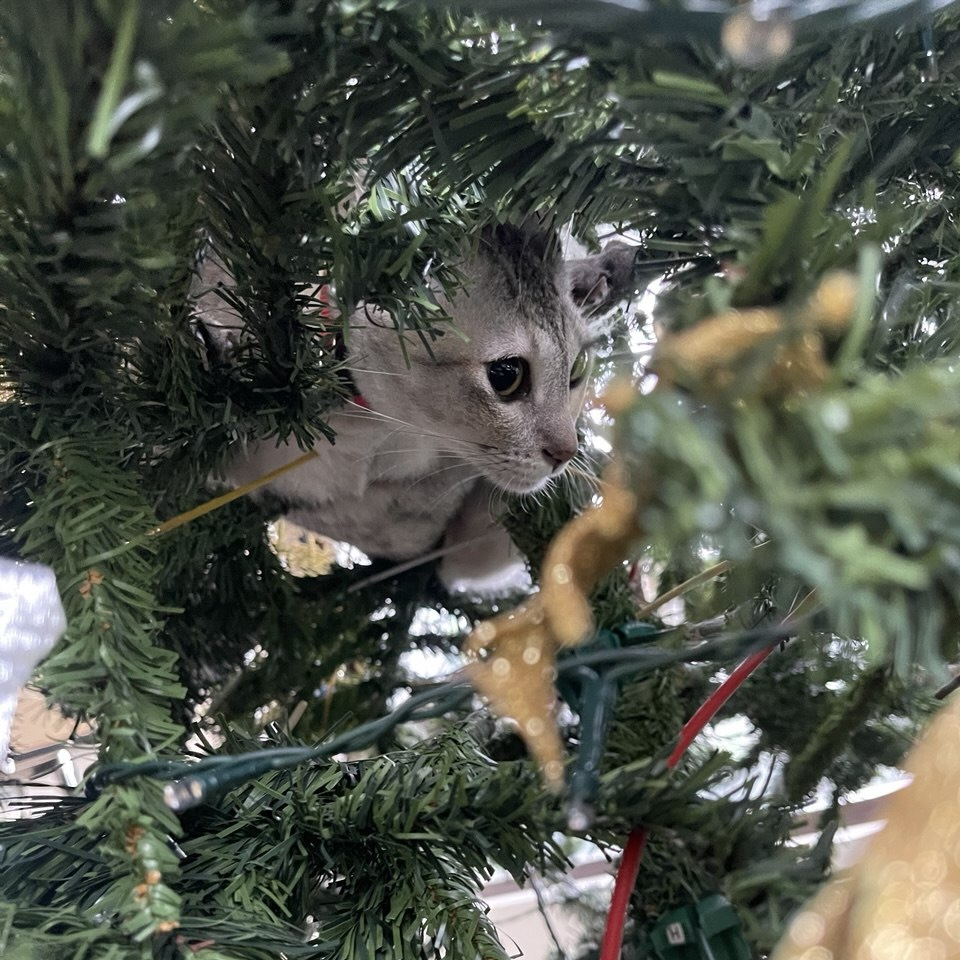
\includegraphics[height=4.4cm]{assets/ash_in_tree.jpg}
    }
    \vspace*{-0.3cm}
    \uncover<3->{
      \caption{My cat, \emph{Ash}, playing with circuit-related
      things\ldots~\textless3}
    }
    \label{fig:ash-in-tree}
  \end{figure}
}

\frame{
  \frametitle{Types of Reduction Problems}
  Let $G = (V, E)$ be a graph with $\lvert V \rvert = n$ nodes,
  $\lvert E \rvert = m$ edges.

  \begin{itemize}
      \uncover<2->{
      \item \emph{Bandwidth recognition:} For a fixed $k$, determine
        whether there exists a layout $\pi$ of $G$ with $\beta(G,
        \pi) \le k$ --- $O(n^k)$
      }
      \uncover<3->{
      \item \emph{Bandwidth minimization:} Find a layout $\pi$ of $G$
        that minimizes (or gets close to minimizing) $\beta(G, \pi)$
        \begin{itemize}
          \item \emph{Exact algorithms:} Find a layout $\pi$ of $G$
            that truly minimizes $\beta(G, \pi)$ --- NP-complete
          \item \emph{(Meta)heuristic algorithms:} Find a layout
            $\pi$ of $G$ that approximately minimizes $\beta(G, \pi)$
            --- typically $O(mn)$ or $O(n^3)$
        \end{itemize}
      }
  \end{itemize}
}

%%%%%%%%%%%%%%%%%%%%%%%%%%%%%%%%%%%%%%%%
\section{Our Contributions}
%%%%%%%%%%%%%%%%%%%%%%%%%%%%%%%%%%%%%%%%
%%%%%%%%%%%%%%%%%%%%%%%%%%%%%%%%%%%%%%%%
\subsection{An Open-Source Interface}
%%%%%%%%%%%%%%%%%%%%%%%%%%%%%%%%%%%%%%%%
\frame{
  \frametitle{Open-Source Interface}
  \begin{itemize}
    \item In open-source, only \emph{reverse Cuthill-McKee} (older,
      less efficient heuristic algorithm from 1971) is widely available
      \uncover<2->{
      \item In \emph{industry}: Want to apply performant modern alternatives
      }
      \uncover<2->{
      \item In \emph{academia}: Want to benchmark new algorithm
        ideas; often also need recognition/exact minimization (e.g.,
        to bound a density matrix's factor width in quantum information theory)
      }
      \uncover<3->{
      \item I have created
        \emph{MatrixBandwidth.jl}\textsuperscript{*}, a unified Julia
        interface for recognition, exact minimization, and
        (meta)heuristic minimization algorithms for bandwidth reduction
      }
      \uncover<4->{
      \item Now using it to investigate \emph{partial layout priority
        heuristics} for bandwidth recognition algorithms\ldots
      }

      \vspace*{1.3cm}
      \uncover<3->{
        \footnotesize{\textsuperscript{*}Available on the official
          Julia package registry and at
        \url{https://www.github.com/Luis-Varona/MatrixBandwidth.jl}}
      }
  \end{itemize}
}

%%%%%%%%%%%%%%%%%%%%%%%%%%%%%%%%%%%%%%%%
\subsection{Partial Layout Priority Heuristics}
%%%%%%%%%%%%%%%%%%%%%%%%%%%%%%%%%%%%%%%%
\frame{
  \frametitle{Base Recognition Algorithm}
  \begin{defn}[Partial layout]
    Let $G = (V, E)$ be a graph. A \emph{partial layout} of $G$ is a
    bijection from $U \bij \{0, 1, \ldots, m - 1\}$ for some $U
    \subseteq V$ with $\lvert U \rvert = m$.
  \end{defn}

  \uncover<2->{
    Base $O(n^k)$ Saxe--Gurari--Sudborough algorithm to find a $\pi$
    with $\beta(G, \pi) \le k$ [Journal of Algorithms \textbf{5}
    (1984), no. 4, 531--46]:
  }

  \begin{enumerate}
      \uncover<3->{
      \item If $G$ violates an $O(n^3)$ ``density'' lower bound,
        return \texttt{null}.
      }
      \uncover<4->{
      \item Initialize an empty queue $Q$ for partial layouts of $G$
        and insert the empty partial layout $\varphi : \emptyset \to \emptyset$.
      }
      \uncover<5->{
      \item While $Q$ is not empty: Extract a partial layout
        $\varphi$ from $Q$.\textsuperscript{*} If $\varphi$ is a full
        layout, return $\varphi$. If $\varphi$ does not violate
        certain constraints, extend it by one node to $\varphi'$ and
        insert $\varphi'$ into $Q$.
      }
      \uncover<6->{
      \item If $Q$ is emptied, return \texttt{null}.
      }
  \end{enumerate}

  \vspace*{0.2cm}
  \uncover<5->{
    \footnotesize{\textsuperscript{*}Step $3$ is simplified
      here---state data associated with each partial layout is also
    stored in $Q$, used to validate bandwidth constraints. (See next slide.)}
  }
}

\frame{
  \frametitle{Adding a Priority Queue (Pt. 1)}
  We can replace the queue of partial layouts with a \emph{min-heap
  priority queue} to find a bandwidth-$k$ layout faster. Associate
  with each partial layout $\varphi : U \bij \{0, 1, \ldots, m - 1\}$
  a $4$-tuple \emph{state} of the form $(\texttt{placed},
  \texttt{unplaced}, \texttt{region}, \texttt{latest})$:
  \begin{enumerate}
      \uncover<2->{
      \item \emph{\texttt{placed}} is an array representation of the
        mapping (i.e., $\texttt{placed}[i] = v$ implies $\varphi(v) = i$)
      }
      \uncover<3->{
      \item \emph{\texttt{unplaced}} is a hash set consisting of the
        nodes in $V \setminus U$ with which we may extend $\varphi$
        to a full layout
      }
      \uncover<4->{
      \item \emph{\texttt{latest}} is a hash map from each node $v
        \in V \setminus U$ to the latest position $i \in \{m, m + 1,
        \ldots, n - 1\}$ it can occupy without violating the
        bandwidth-$k$ constraint
      }
      \uncover<5->{
      \item \emph{\texttt{region}} is a another data structure
        tracking edges connecting $U$ to $V \setminus U$, used to
        validate bandwidth constraints in Step $3$
      }
  \end{enumerate}
}

\frame{
  \frametitle{Adding a Priority Queue (Pt. 2)}
  We use MatrixBandwidth.jl to compare three \emph{priority functions}
  for a state $s$, adapted from \emph{constraint satisfaction problems}:
  \begin{itemize}
      \uncover<2->{
      \item \emph{Least-active-nodes} heuristic:
        \footnotesize{
          \begin{align*}
            \texttt{priority}_{\texttt{lan}}(s) = \left\lvert
            \bigl\{v \in s.\texttt{unplaced} : \exists u \in
            s.\texttt{placed} \text{ with } \{u, v\} \in E\bigr\} \right\rvert
          \end{align*}
        }
        \normalsize{}
      }
      \uncover<3->{
      \item \emph{Minimum-remaining-values} heuristic:
        \footnotesize{
          \begin{align*}
            \texttt{priority}_{\texttt{mrv}}(s) =
            \min\bigl\{s.\texttt{latest}[v] - \lvert
            s.\texttt{placed} \rvert : v \in s.\texttt{unplaced}\bigr\}
          \end{align*}
        }
        \normalsize{}
      }
      \uncover<4->{
      \item \emph{Total-remaining-values} heuristic:
        \footnotesize{
          \begin{align*}
            \texttt{priority}_{\texttt{trv}}(s) = \sum_{v \in
            s.\texttt{unplaced}}\bigl(s.\texttt{latest}[v] - \lvert
            s.\texttt{placed} \rvert\bigr)
          \end{align*}
        }
      }
  \end{itemize}
}

%%%%%%%%%%%%%%%%%%%%%%%%%%%%%%%%%%%%%%%%
\section{Conclusions and Future Work}
%%%%%%%%%%%%%%%%%%%%%%%%%%%%%%%%%%%%%%%%
%%%%%%%%%%%%%%%%%%%%%%%%%%%%%%%%%%%%%%%%
\subsection{Next Steps}
%%%%%%%%%%%%%%%%%%%%%%%%%%%%%%%%%%%%%%%%
\frame{
  \frametitle{Next Steps}
  \begin{figure}
    \centering
    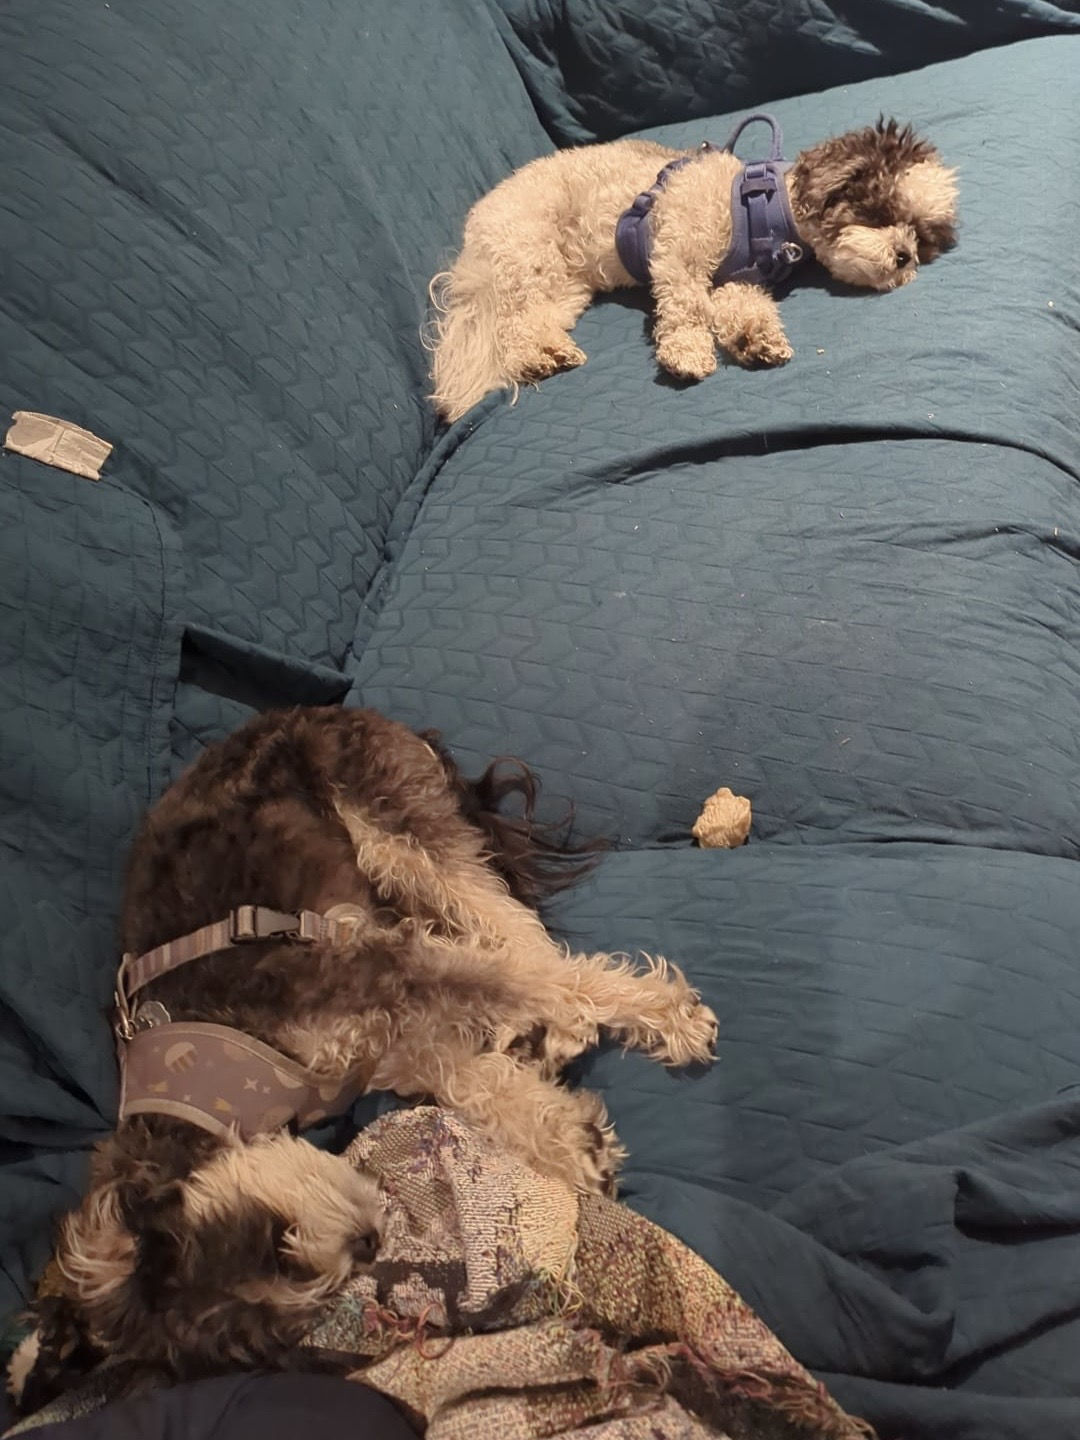
\includegraphics[height=6.9cm]{assets/jonsi_and_timmy.jpg}
    \vspace*{-0.3cm}
    \caption{Rebekka's dogs, \emph{Jonsi} (right) and \emph{Timmy}
    (left), being cute \textless3}
    \label{fig:jonsi-and-timmy}
  \end{figure}
}

%%%%%%%%%%%%%%%%%%%%%%%%%%%%%%%%%%%%%%%%
\subsection{Thank you!}
%%%%%%%%%%%%%%%%%%%%%%%%%%%%%%%%%%%%%%%%
\frame{
  \frametitle{Thank you!}
  \begin{figure}
    \centering
    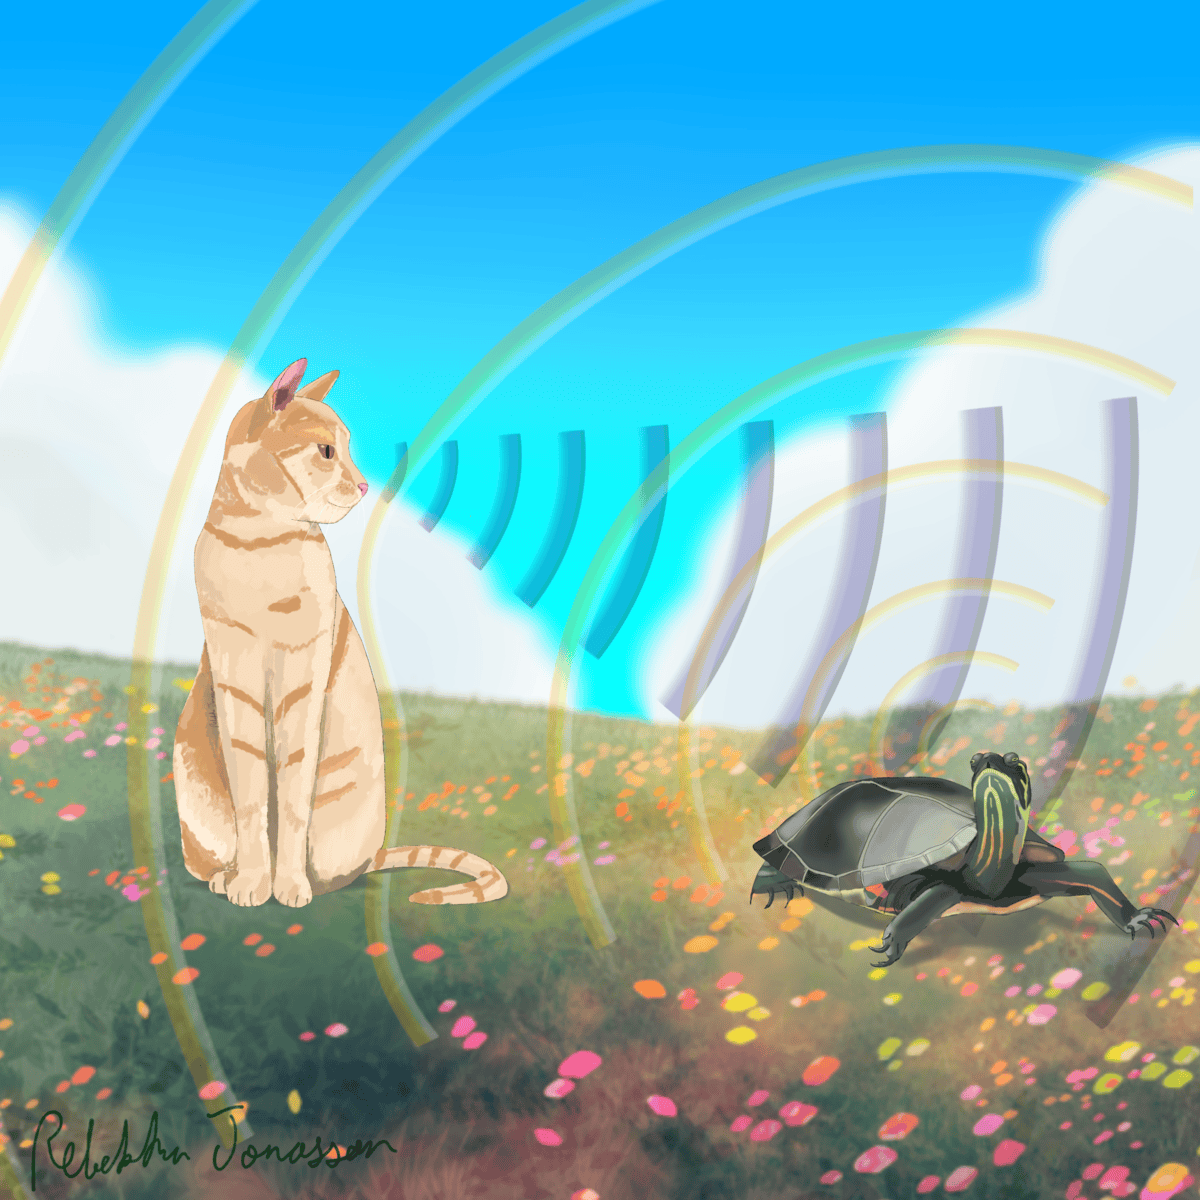
\includegraphics[height=6.9cm]{assets/matband_logo.png}
    \vspace*{-0.3cm}
    \caption{Art by \emph{Rebekka Jonasson} \textless3}
    \label{fig:matband-logo}
  \end{figure}
}
\end{document}
